\documentclass[10pt]{article}\usepackage[margin=.55in]{geometry}\usepackage[T1]{fontenc}\usepackage{graphicx}\setlength{\parindent}{0pt}\setlength{\parskip}{4pt}\sloppy\begin{document}{\large Finite-difference integration in the actual producer}\par Integrated the independently reviewed finite-difference candidate into the actual native producer source. The exact tested bytes now occupy research/pencil\_large\_prime\_20261029/src/native\_solver.rs. The production change replaces only the two per-x Horner evaluations; the original baseline and paired controls are retained in a cfg(test) module.\par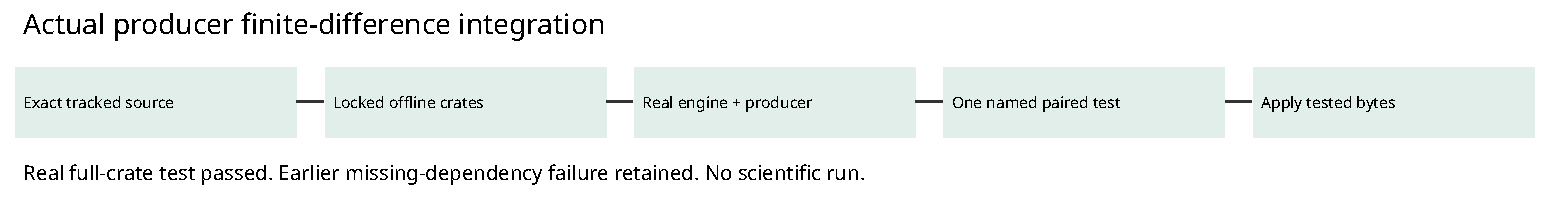
\includegraphics[width=.96\linewidth]{diagram.pdf}\par The final ordinary check compiled the real five-leads-study engine and pencil-symbolic-graph producer library with offline, locked dependencies and one build job. Exactly one named test passed, with 6,398 complete result pairs, 20,207 arithmetic sequences at 134,067 points, 32 boundary transitions and three incorrect-recurrence controls. The wrapper verified ordered pair IDs and the exact branch-coverage summary, preventing a zero-test filter success.

The candidate and baseline agree on candidate sets, scalar result counters and ordered buckets. Real arithmetic and symbolic counters satisfy the exact recorded deltas. Active-slice padding and advance-before-continue are retained. Low-degree addition increases remain part of the result; no timing speedup is claimed.

The first integration attempt stopped before tests after 8.065760 seconds because the private closure omitted the transitive three\_leads\_constructor\_primality.rs dependency. That preparation failure, source freeze and logs are preserved. The separately authorized successor added its exact tracked Git bytes and audited all 16 selected path/mod/include edges. It passed in 11.544328 seconds with unchanged frozen inputs and a reaped command process. No automatic retry followed either attempt.

The corrected private closure contains actual source types and derives, unlike the earlier extraction harness. Twelve dependency archives matched the existing Cargo.lock checksums and were unpacked into a private offline vendor tree. The single successor envelope was 240 seconds including kill grace, 4 GiB address space and one build job. Source hash 061f4f9f45d261b61af3482509ca5f09e03964abc670765852922d20f946bbd1 binds the tested and applied canonical bytes.

Independent component review ec66714bf904a3bbde089a65cfbe3537a7229b498860ccf758d6516af03cd0fc accepted the source-extraction candidate and scoped Lean evidence. The proved ring iteration and separate canonical UInt64 addition do not yet compose into a complete iterative word-refinement theorem. Current coverage/pricing classification for Option/bounds/scalar-copy behavior and a fresh scientific protocol/source/binary binding remain separate gates. This packet contains ordinary software tests only.
\end{document}